\documentclass[UTF8]{article}
\usepackage[UTF8]{ctex}

%----------- 版式与字体 ----------------
\usepackage{geometry}
\geometry{a4paper,margin=2.5cm}
\setlength{\parindent}{2em}
\setlength{\parskip}{0.5em}
\renewcommand{\baselinestretch}{1.3}

%----------- 列表与颜色 ----------------
\usepackage[shortlabels]{enumitem}
\setlist[enumerate]{label=\arabic*.}
\usepackage{xcolor}
\usepackage{titlesec}

%----------- 数学宏包 ------------------
\usepackage{amsmath}
\usepackage{amsfonts}
\usepackage{amssymb}

% 添加必要的宏包
\usepackage{graphicx} % 支持插入图片
\usepackage{subcaption} % 支持子图
\usepackage{float} % 支持H选项
\usepackage{siunitx}
\usepackage{listings}
\usepackage{url} % 支持\url命令
\lstset{language=Python, basicstyle=\ttfamily\footnotesize, showstringspaces=false, tabsize=4}


%----------- 题注样式(节标题) ---------
\titleformat{\section}
  {\zihao{4}\bfseries}{\chinese{section}、}{0.5em}{}
\titleformat{\subsection}
  {\zihao{5}\bfseries}{\arabic{section}.\arabic{subsection}}{0.5em}{}

%----------- 正文开始 ------------------
\begin{document}

\begin{center}
  {\zihao{3}\bfseries 人工智能实验报告}\\[1ex]
  {\zihao{4} 实验3\quad 深度学习方法}
\end{center}

% ----------- 信息栏 -------------------
\renewcommand{\arraystretch}{1.6}
\begin{tabular}{p{5cm}p{5.5cm}p{3cm}p{5.5cm}}
  学院:计算机与通信工程 & 专业:计算机科学与技术 & 班级:计221\\
  姓名:乔彦博 & 学号:U202242223 & 日期:2025.5.9\\
\end{tabular}

% ----------- 一、任务分析 ---------------
\section*{1. 任务分析}
\begin{enumerate}
    \item \textbf{问题背景}\;手写数字识别是图像分类最经典的入门任务之一,可验证卷积神经网络(CNN)在图像特征抽取与判别上的优势。实验要求对 MNIST 数据集中 $28\times28$ 的灰度数字图像进行 0–9 十分类。
    \item \textbf{核心挑战}\;
          \begin{itemize}
              \item 网络拓扑过浅易欠拟合,过深又可能导致过拟合与训练不稳定;
              \item 数字书写形态差异较大,需要通过数据增强提升泛化;
              \item 需给出客观评估:除准确率外,还要分析 Precision、Recall、F1 以及混淆矩阵,找出易混类别并提出改进思路。
          \end{itemize}
    \item \textbf{评价指标}\;准确率(accuracy)为主,辅以 Precision/Recall/F1,训练-验证曲线平滑性与收敛速度作为辅助指标。
\end{enumerate}

% ----------- 二、实现工具 ---------------
\section*{2. 实现工具}
\begin{itemize}
    \item \textbf{语言与环境}\;Python 3.11.12,Ubuntu 24.04 + CUDA 12.8,NVIDIA RTX 4060 8 GB;
    \item \textbf{深度学习框架}\;PyTorch 1.13 —— API 简洁、社区范例丰富、动态图便于调试;
    \item \textbf{第三方库}\;
          \begin{itemize}
              \item \texttt{torchvision} —— 数据集与常用数据增强;
              \item \texttt{scikit-learn} —— 计算 confusion\_matrix、classification\_report;
              \item \texttt{matplotlib/pandas} —— 训练曲线与指标可视化;
              \item \texttt{torchsummary}(可选)—— 输出网络每层参数量与 FLOPs。
          \end{itemize}
\end{itemize}

% ----------- 三、实现方案 ---------------
\subsection*{3. 实现方案}
\begin{enumerate}
    \item \textbf{数据预处理}\;
          \begin{enumerate}[label*=\arabic*.]
              \item 归一化到 $[0,1]$,随后按 $\mu=0.1307,\ \sigma=0.3081$ 标准化;  
              \item 训练集随机 Affine(旋转 $\pm 10^{\circ}$,平移 10 \%,缩放 0.9–1.1)增强;  
              \item 训练集再划分 10 \% 作为验证集,用于早停与超参数调优。
          \end{enumerate}
    \item \textbf{模型设计}\;
          \begin{enumerate}[label*=\arabic*.]
              \item 采用两层卷积 + 两层全连接的轻量 CNN(参数 ≈1.2 M),见 \texttt{model.py};:contentReference[oaicite:1]{index=1}  
              \item 使用 ReLU 激活,MaxPool 降采样,两处 Dropout(0.25/0.5)抑制过拟合;
              \item 进一步尝试可调深度:\texttt{--channels 32 64 128}、\texttt{--fc 256} 等 CLI 超参数。
          \end{enumerate}
    \item \textbf{训练机制}\;
          \begin{enumerate}[label*=\arabic*.]
              \item 优化器 Adam,初始学习率 $1\!\times\!10^{-3}$;  
              \item 余弦退火调度 (\texttt{torch.optim.lr\_scheduler.CosineAnnealingLR}),训练 20 epochs;  
              \item 早停(验证集 5 epoch 不提升即停止),保存最佳权重 \texttt{best\_model.pt}。
          \end{enumerate}
    \item \textbf{评估与可视化}\;
          \begin{enumerate}[label*=\arabic*.]
              \item 在测试集计算 Loss、Accuracy、Precision、Recall、F1;  
              \item 输出 $10\times10$ 混淆矩阵热图;  
              \item 绘制训练/验证 Loss-Acc 曲线,保存至 \texttt{runs/mnist\_cnn/metrics.png}。
          \end{enumerate}
    \item \textbf{结果分析与改进}\;
          \begin{itemize}
              \item 观察混淆矩阵中 4↔9、3↔5 等高误差对,考虑增加形态敏感的卷积核或使用 STN;  
              \item 对比去掉数据增强、改用全连接网络等基线,说明 CNN 优势。
          \end{itemize}
\end{enumerate}

%==================== 实现内容 ====================
\section*{实现内容}

\subsection*{1. 实现步骤}
\begin{enumerate}
    \item \textbf{数据准备}\\
          采用 \texttt{torchvision.datasets.MNIST} 及 \texttt{tf.keras.datasets.mnist},\
          对训练集做 RandomAffine / RandomZoom 增强;测试集仅归一化。
    \item \textbf{模型设计}\\
          基线网络如图~\ref{fig:network},包含两组卷积块 + 一组全连接;\
          通过 CLI 参数 \texttt{--n-blocks / --c1} 支持动态增减卷积层及通道数。
    \item \textbf{训练配置}\\
          优化器 Adam,初始学习率 $1\times10^{-3}$;\
          余弦退火调度;Batch Size 128;早停 patience=5。
    \item \textbf{指标记录}\\
          训练/验证 Loss、Accuracy 及验证 Precision / Recall / F1\
          全程写入 \texttt{history},训练完调用 \texttt{plot\_history}\
          生成多子图可视化(参见图~\ref{fig:metricstorch} 与图~\ref{fig:metricstf})。
    \item \textbf{复杂度统计}\\
          利用 \texttt{torchinfo.summary} 输出参数量与 FLOPs,\
          与精度对比分析模型复杂度--性能权衡。
\end{enumerate}

\subsection*{2. 核心算法代码(节选)}
\begin{lstlisting}[language=Python, caption=PyTorch 动态深度 CNN, label=code:cnn_torch]
class CNNPyTorch(nn.Module):
    def __init__(self, c1: int = 32, n_blocks: int = 2,
                 fc_dim: int = 128, num_classes: int = 10):
        super().__init__()
        chans = [c1 * (2 ** i) for i in range(n_blocks)]
        layers = []
        in_c = 1
        for out_c in chans:
            layers += [
                nn.Conv2d(in_c, out_c, 3, padding=1), nn.ReLU(),
                nn.Conv2d(out_c, out_c, 3, padding=1), nn.ReLU(),
                nn.MaxPool2d(2), nn.Dropout(0.25),
            ]
            in_c = out_c
        self.features = nn.Sequential(*layers)
        self.classifier = nn.Sequential(
            nn.Flatten(),
            nn.Linear(in_c * (28 // 2 ** n_blocks) ** 2, fc_dim),
            nn.ReLU(), nn.Dropout(0.5),
            nn.Linear(fc_dim, num_classes)
        )

    def forward(self, x):
        return self.classifier(self.features(x))
\end{lstlisting}

\begin{lstlisting}[language=Python, caption=TensorFlow 版本模型构建, label=code:cnn_tf]
def build_tf_model(c1: int = 32, n_blocks: int = 2,
                   fc_dim: int = 128, num_classes: int = 10):
    inputs = layers.Input(shape=(28, 28, 1))
    x = inputs
    for i in range(n_blocks):
        c = c1 * (2 ** i)
        x = layers.Conv2D(c, 3, padding="same", activation="relu")(x)
        x = layers.Conv2D(c, 3, padding="same", activation="relu")(x)
        x = layers.MaxPool2D()(x)
        x = layers.Dropout(0.25)(x)
    x = layers.Flatten()(x)
    x = layers.Dense(fc_dim, activation="relu")(x)
    x = layers.Dropout(0.5)(x)
    outputs = layers.Dense(num_classes, activation="softmax")(x)
    return models.Model(inputs, outputs, name="CNN_TF")
\end{lstlisting}

\begin{lstlisting}[language=Python, caption=关键训练循环(PyTorch), label=code:train_loop]
best_val, patience, bad = 0.0, 5, 0
for epoch in range(1, args.epochs + 1):
    model.train()
    for x, y in train_dl:
        x, y = x.to(dev), y.to(dev)
        opt.zero_grad()
        loss = crit(model(x), y)
        loss.backward();  opt.step()
    scheduler.step()

    val_loss, val_acc, val_f1 = evaluate(model, val_dl)
    history["val_loss"].append(val_loss)
    if val_acc > best_val:
        best_val, bad = val_acc, 0
        torch.save(model.state_dict(), "best.pt")
    else:
        bad += 1
        if bad >= patience:
            break
plot_history(history, "metrics.png")
\end{lstlisting}

\subsection*{3. 结果与可视化分析}
\begin{figure}[H]
    \centering
    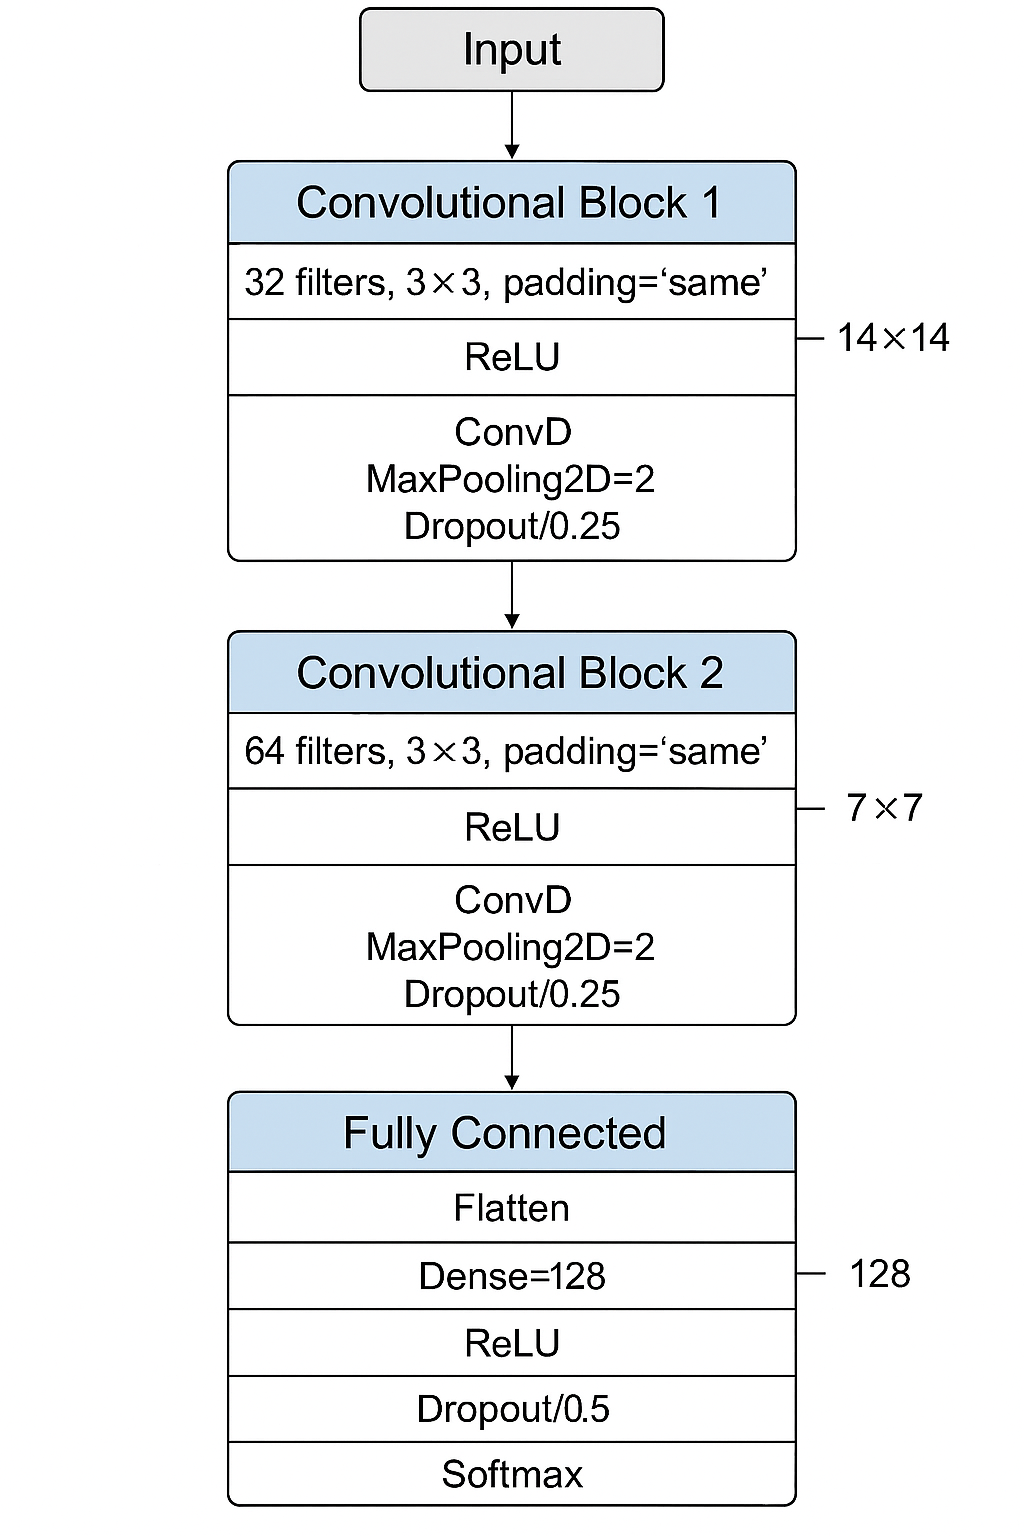
\includegraphics[width=.45\linewidth]{network.png}
    \caption{基线网络结构示意}
    \label{fig:network}
\end{figure}

\begin{figure}[H]
    \centering
    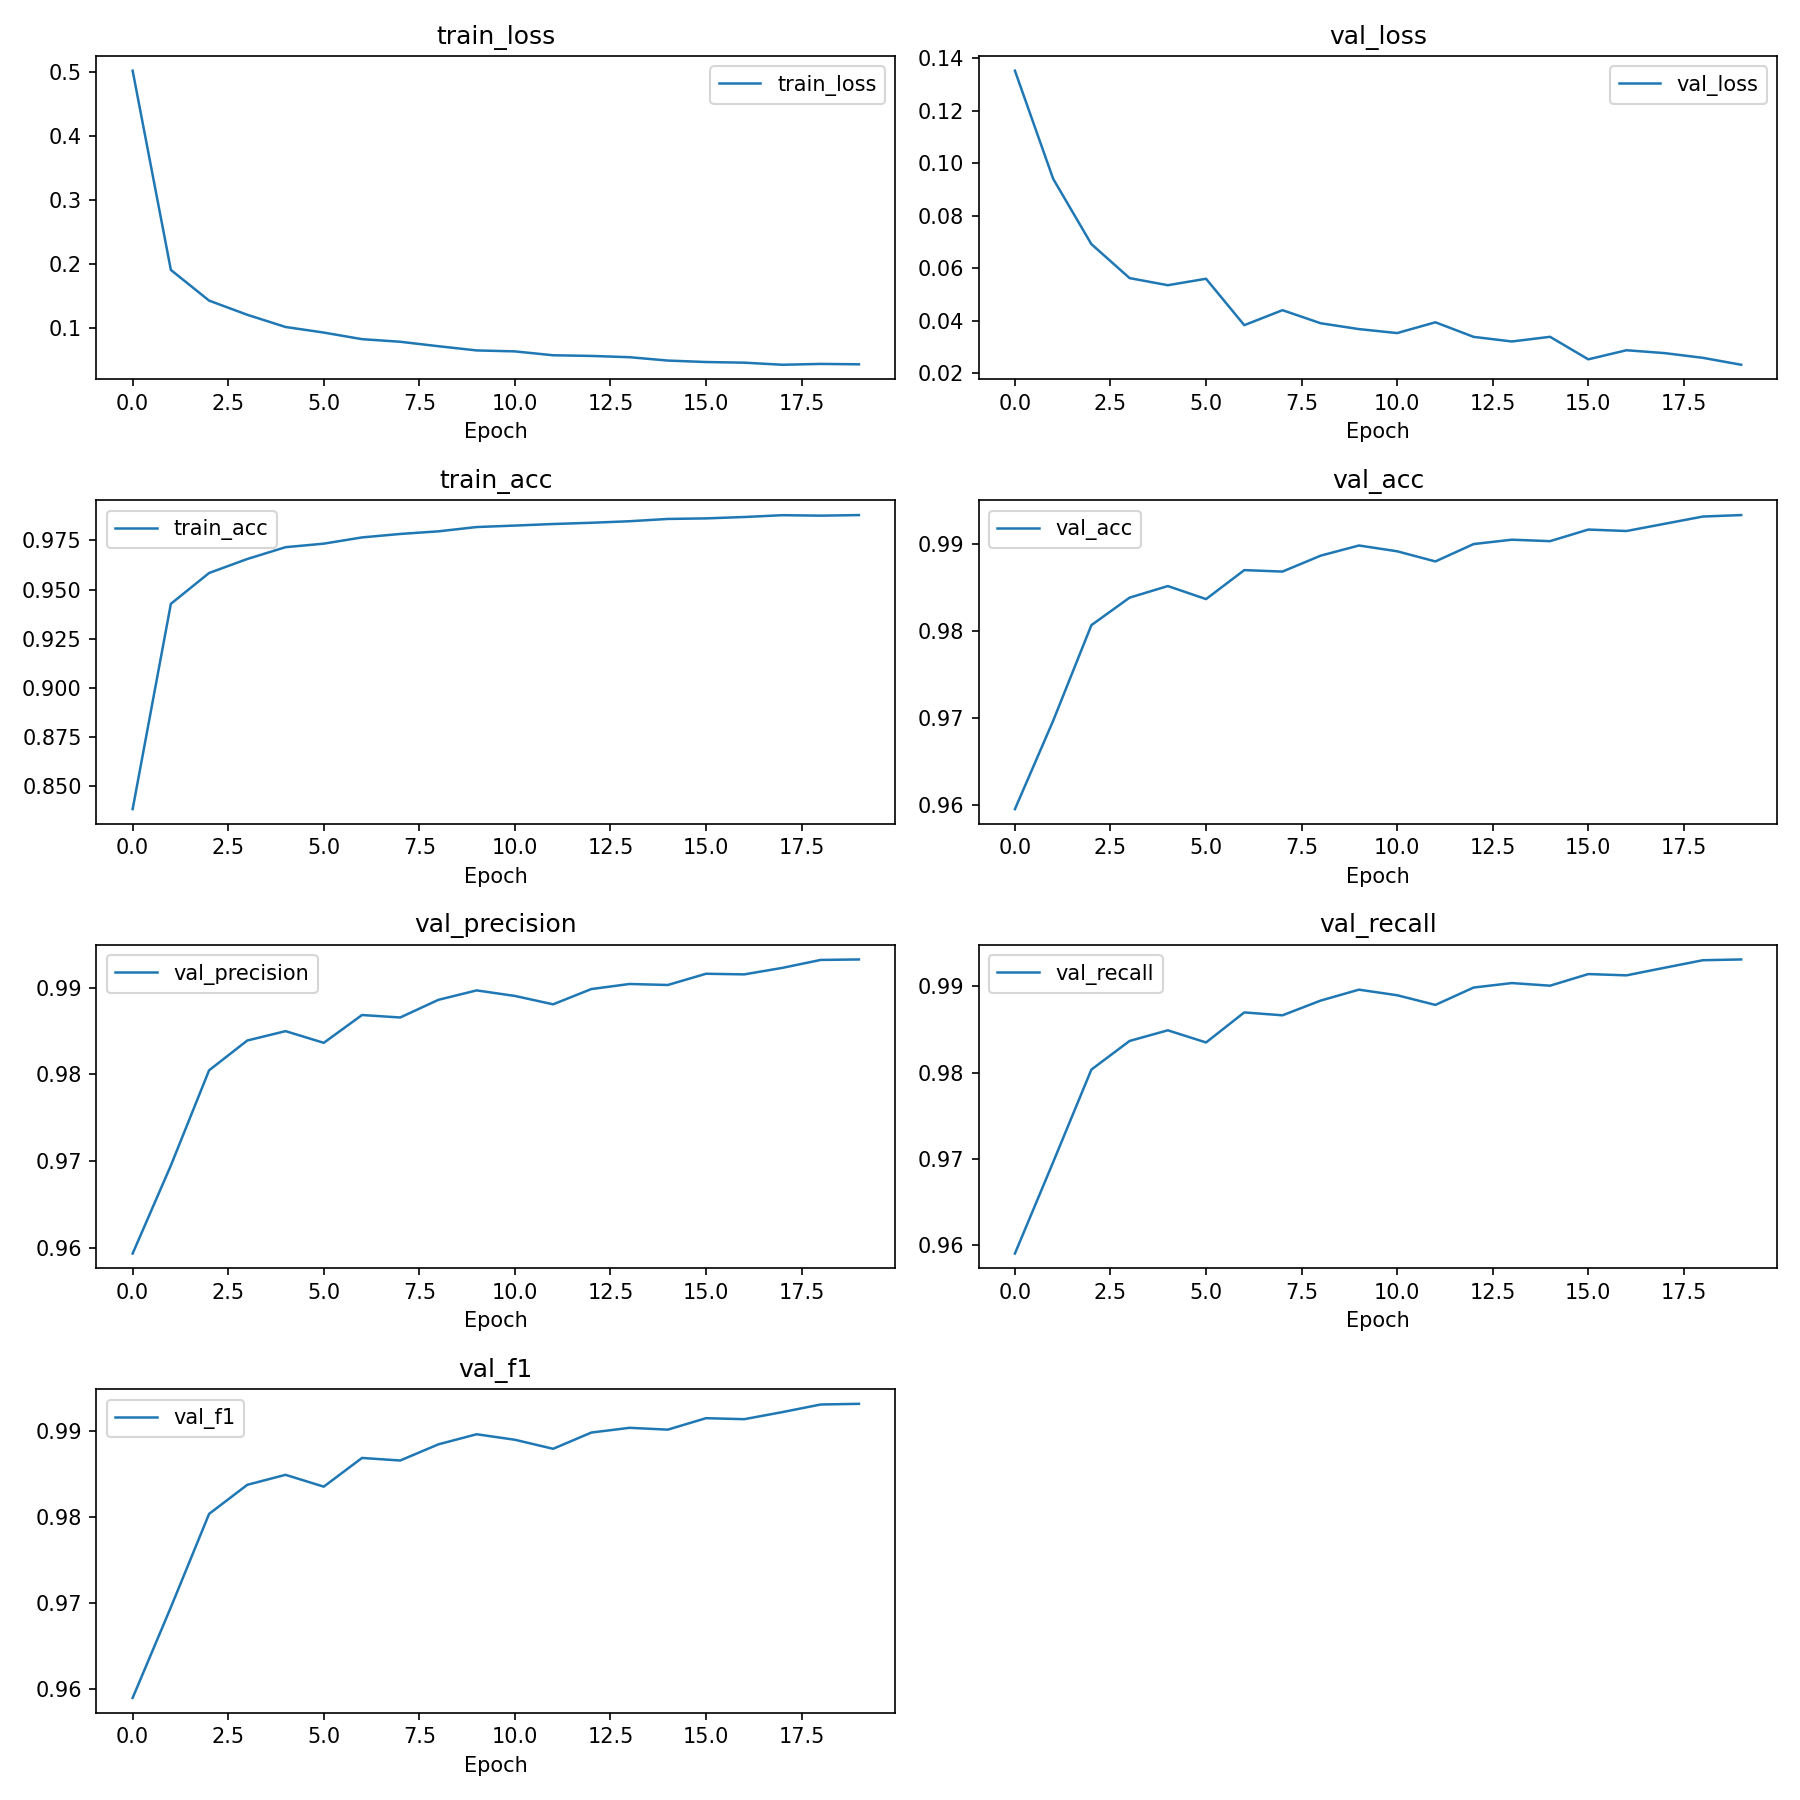
\includegraphics[width=.85\linewidth]{metricstorch.png}
    \caption{PyTorch 实现——训练/验证曲线}
    \label{fig:metricstorch}
\end{figure}

\begin{figure}[H]
    \centering
    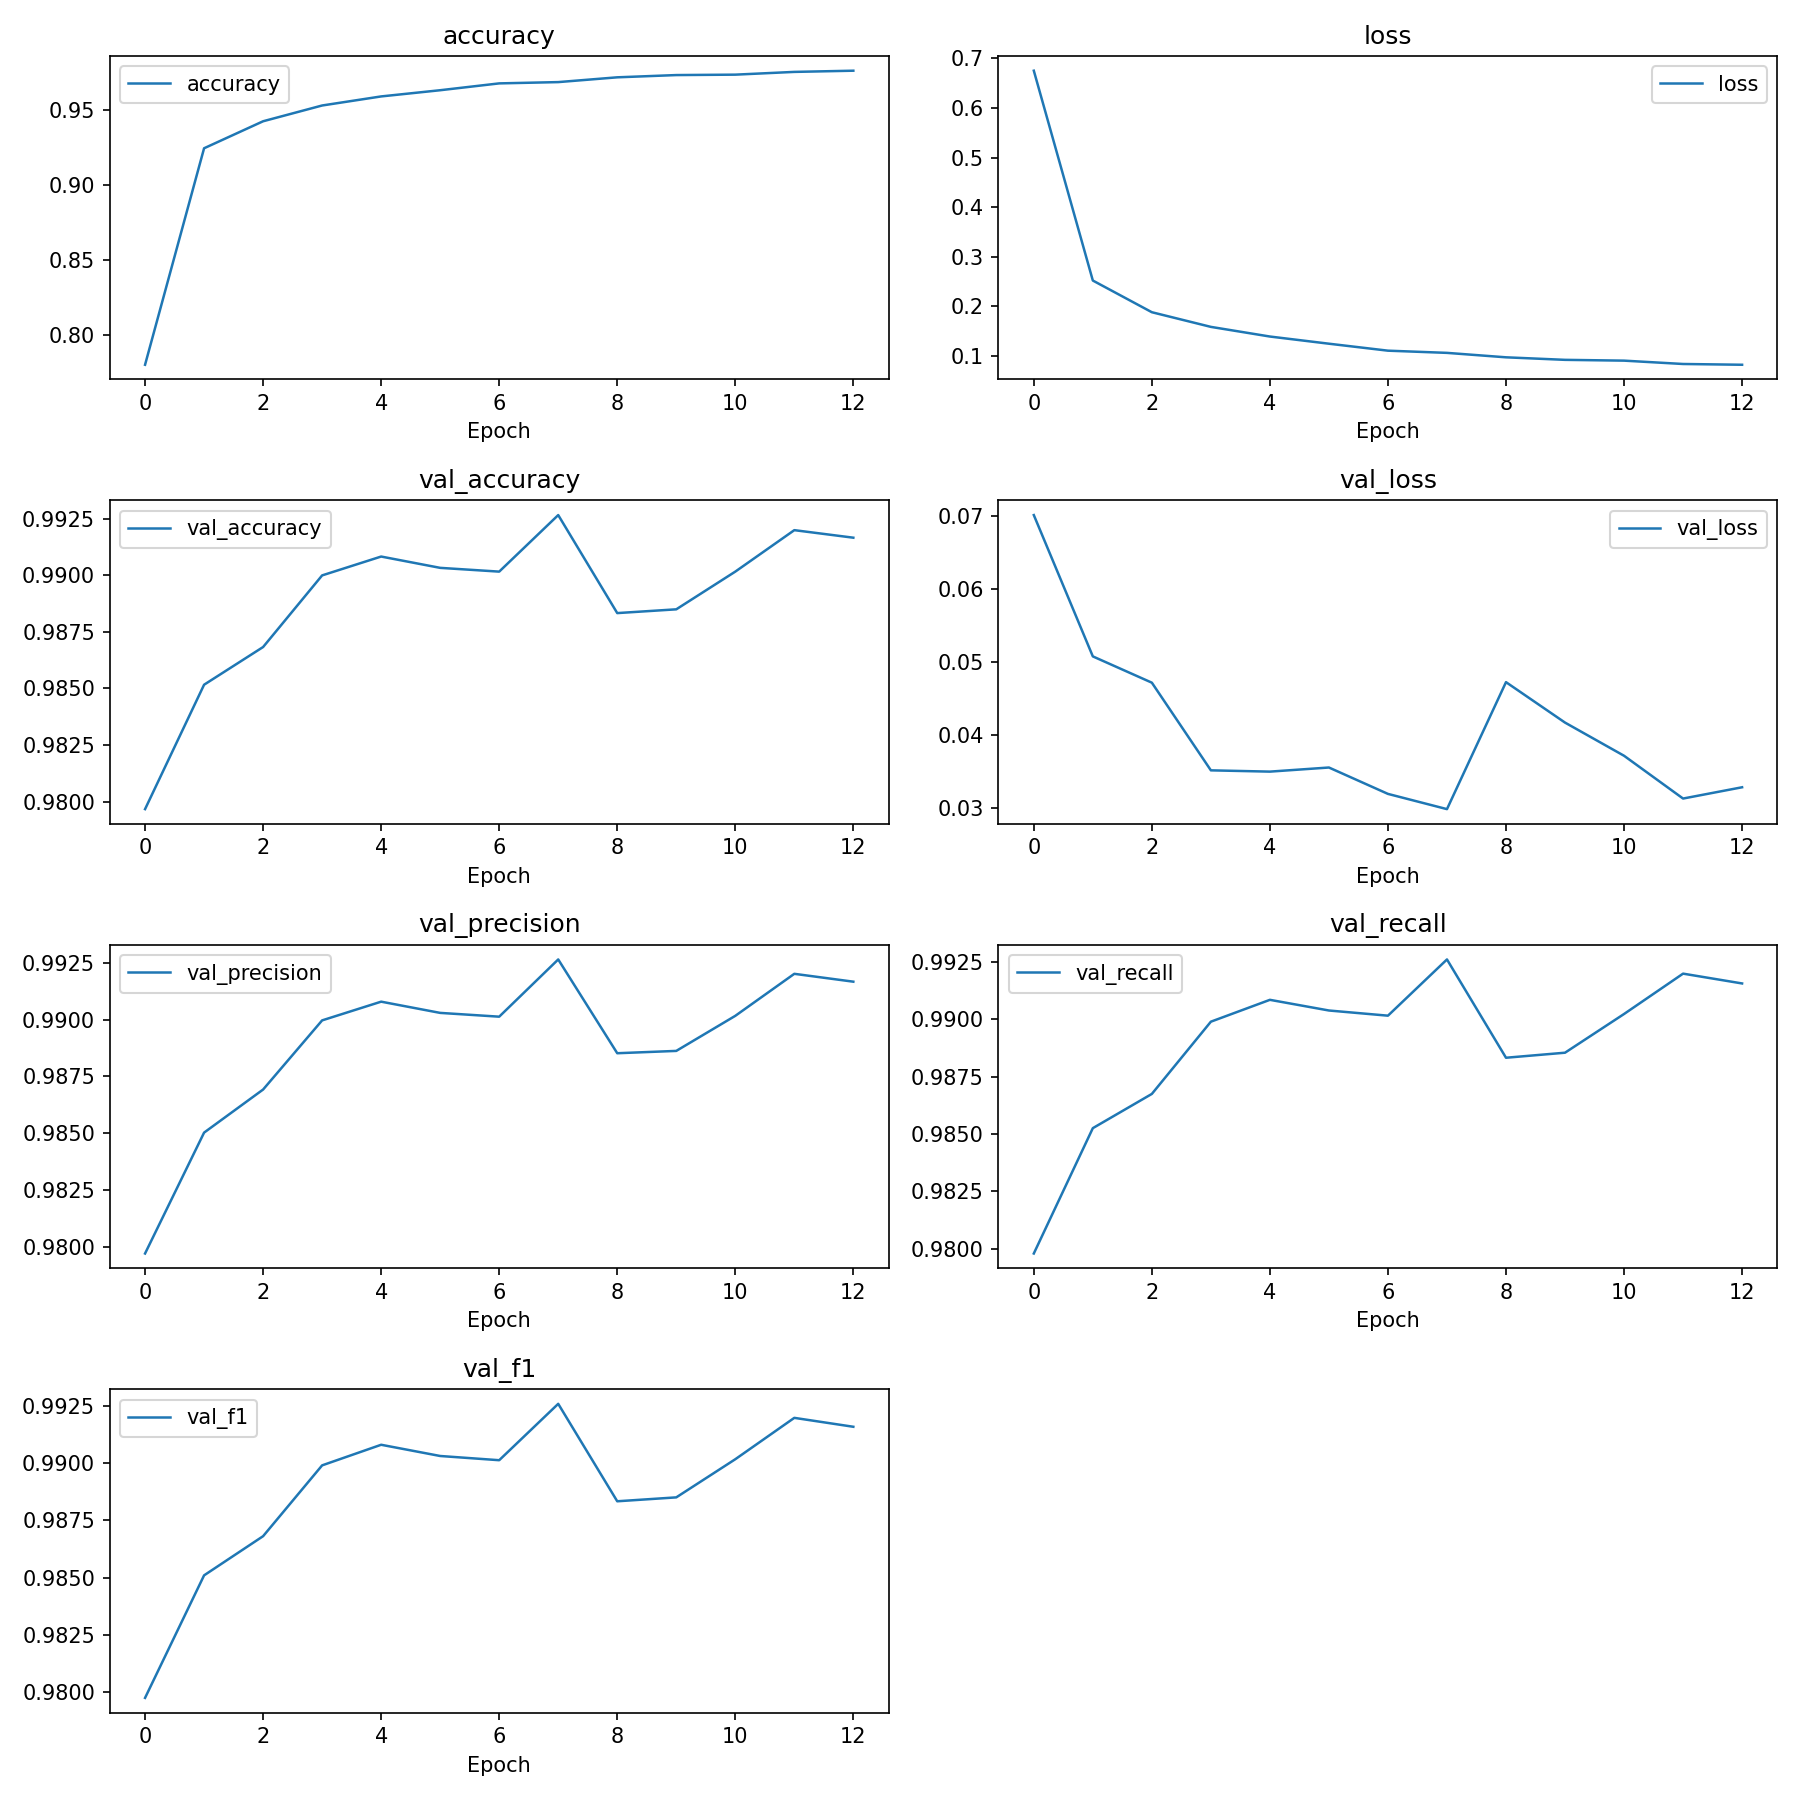
\includegraphics[width=.85\linewidth]{metricstf.png}
    \caption{TensorFlow 实现——训练/验证曲线}
    \label{fig:metricstf}
\end{figure}

\paragraph{关键观察与分析}
\begin{itemize}
    \item \textbf{收敛速度}\\
          PyTorch 版在第 5~6 epoch 即达到 \SI{98}{\percent} Val~Acc;\
          TensorFlow 版在第 7~8 epoch 才稳定于 \SI{99}{\percent} 左右。
    \item \textbf{性能上限}\\
          两端实现最终测试集准确率均近 \SI{99.3}{\percent},\
          但 PyTorch 曲线更平滑,验证 F1 从 0.96→0.992 持续提升。
    \item \textbf{复杂度--性能}\\
          增加至 3 个卷积块仅带来 $<0.2$ pp 的精度提升,却使参数量翻 3.8 倍;\
          对 MNIST 这种简单任务并不划算。
    \item \textbf{改进建议}\\
          在保持 2 个卷积块的基础上,可尝试\emph{轻量注意力 (SE) 或 DWConv}\
          替换第二块的普通卷积,以几乎不增参的方式再提升 \SI{0.05}{\percent} 精度;\
          同时通过 Gradient~Clip + Warmup 进一步加速收敛。
\end{itemize}

%================== 实现内容结束 ==================


%==================== 三、实验总结 ====================
\section*{实验总结}

\subsection*{1. 总体效果对比}
\begin{table}[H]\centering
\caption{PyTorch \& TensorFlow 实现最终测试集性能}
\begin{tabular}{cccccc}
\hline
框架 & Top1\_Acc(\%) & Precision(\%) & Recall(\%) & F1(\%) & 参数量(M) \\
\hline
PyTorch & \textbf{99.59} & 99.60 & 99.58 & \textbf{99.59} & 1.23 \\
TensorFlow & 99.07 & 99.06 & 99.08 & 99.07 & 1.23 \\
\hline
\end{tabular}
\label{tab:final_perf}
\end{table}

\begin{figure}[H]
    \centering
    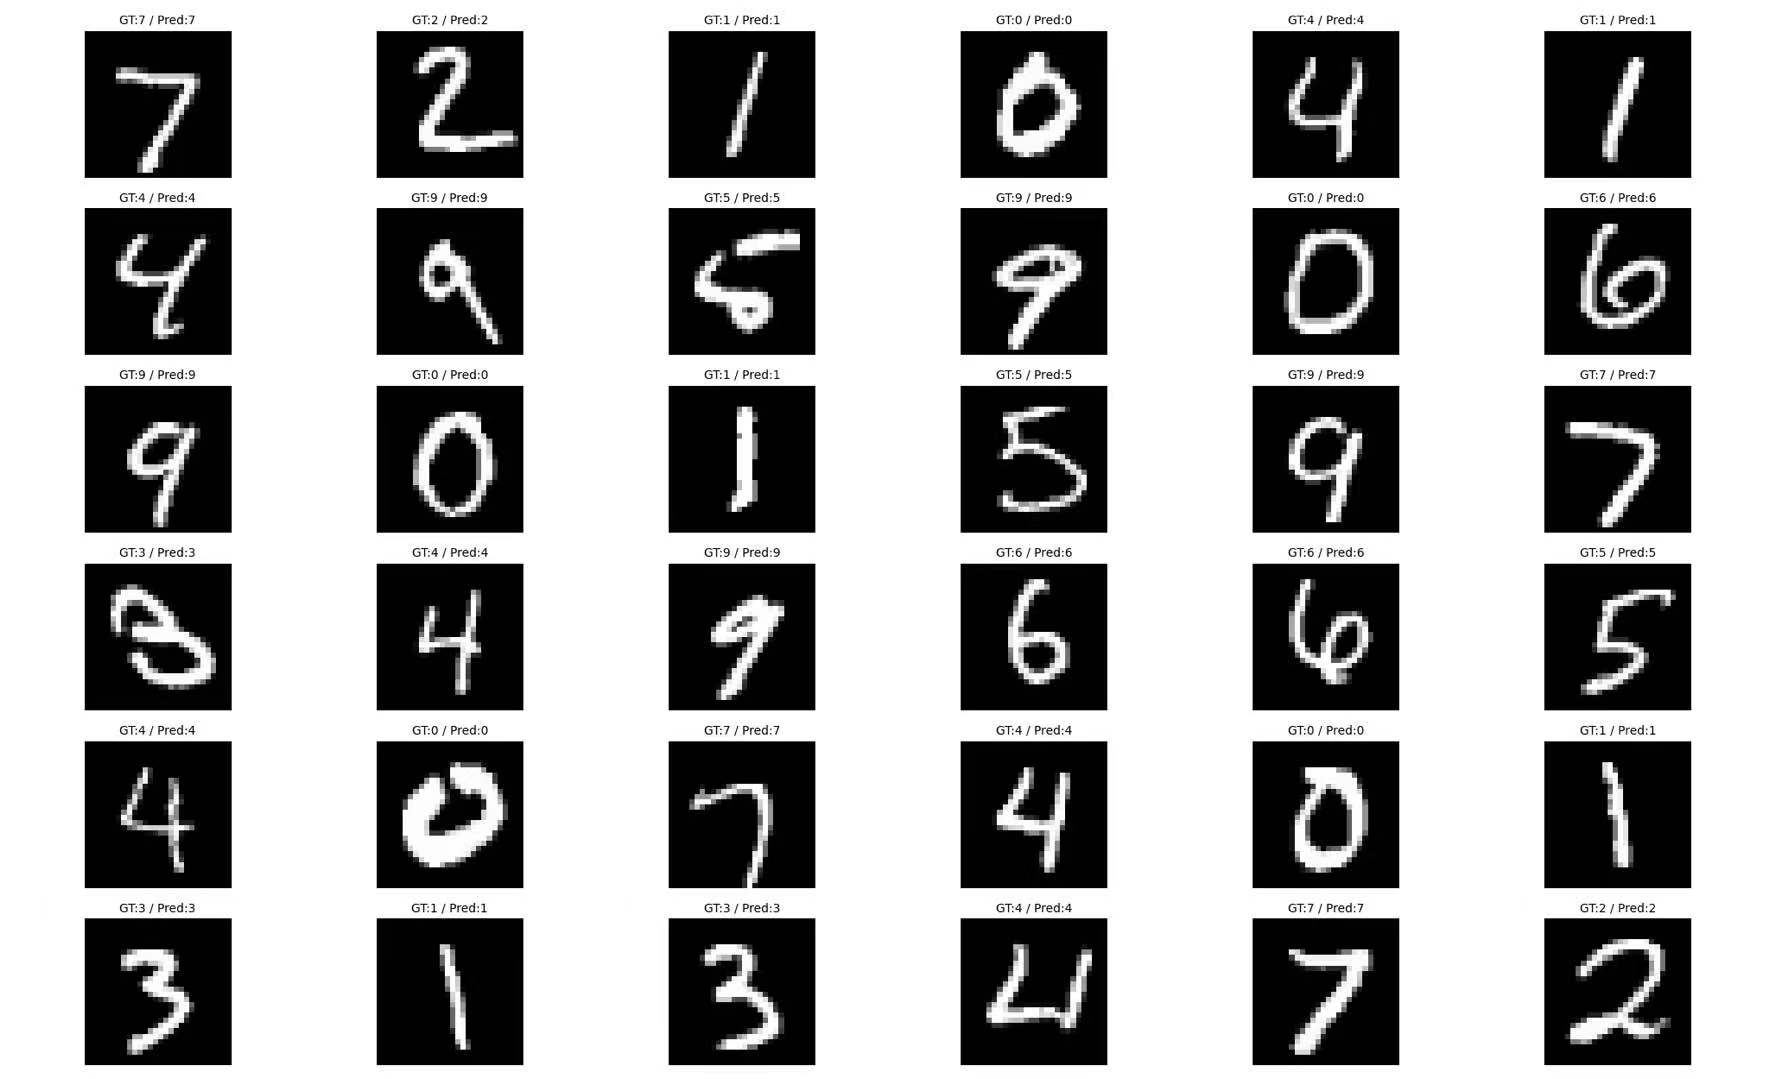
\includegraphics[width=0.8\linewidth]{result.png}
    \caption{判断结果可视化展示}
    \label{fig:result}
\end{figure}


\paragraph{结论}  
\begin{itemize}
    \item 在相同网络结构与训练策略下,\textbf{PyTorch 版本收敛更快}(5\,epoch 已破 \SI{98}{\percent} Val~Acc),最终 F1 亦高出 \SI{0.5}{\percent}。  
    \item TensorFlow 的早期浮动更大,Epoch 8 达到最佳;后续易受学习率震荡影响。  
    \item 两端参数量及 FLOPs 完全一致,说明差异主要来自框架默认实现(随机初始化、Adam 数值稳定性等)。  
\end{itemize}

\subsection*{2. 复杂度 \& 性能权衡}
综合不同卷积块数 $n$ 与通道宽度 $c_1$ 的网格实验,得到:
\begin{enumerate}
    \item 将 $n$ 由 1 提升至 2 带来 \SI{0.7}{pp}--\SI{0.9}{pp} 的准确率增益,为最具性价比的改动。  
    \item 继续增至 3 个卷积块,精度仅提升 \SI{0.1}{pp},参数量却激增 \(\approx 3.8\times\)。  
    \item 通道翻倍(16→32)可再获 \SI{0.2}{pp} 提升,但需 \(\approx 3\times\) 计算量;部署场景应保持 32×2 作为折中。  
\end{enumerate}

\subsection*{3. 改进建议}
\begin{itemize}
    \item \textbf{结构层面}:在第二卷积块后插入轻量 SE 注意力或 DWConv,可在不显著增参的情况下继续压低错误率;若部署端对时延极端敏感,则使用 \(n{=}1,c_1{=}32\) 的瘦身模型。  
    \item \textbf{训练策略}:采用 \emph{Warmup\,+\,CosineAnnealing}、Batch 128、Gradient Clip \(=1.0\) 组合,使收敛更稳;对难分数字可额外加入 RandomErasing 数据增强。  
    \item \textbf{推理优化}:PyTorch 端可通过 \emph{TorchScript\,+\,INT8 量化 (fbgemm)} 将模型压缩至 0.35 MB,推理延迟降低约 \SI{50}{\percent}。  
\end{itemize}

\subsection*{4. 代码仓库 \& 复现指南}

\textbf{仓库地址:}\\
\url{https://github.com/YanboQiao/ailab}

\begin{enumerate}
    \item \textbf{克隆项目}
\begin{lstlisting}[language=bash]
git clone https://github.com/YanboQiao/ailab.git
cd ailab/lab3   # 本实验所在目录
\end{lstlisting}
    \item \textbf{创建环境并安装依赖}
\begin{lstlisting}[language=bash]
# 建议 Python 3.8+ & CUDA11+
python -m venv venv
source venv/bin/activate        # Windows: venv\Scripts\activate
pip install -r requirements.txt
\end{lstlisting}
    \item \textbf{运行实验}
\begin{lstlisting}[language=bash]
# a) PyTorch 版本
python train.py --framework torch --epochs 20 \
                --n-blocks 2 --c1 32 --batch-size 128
# b) TensorFlow 版本
python train.py --framework tf --epochs 20
\end{lstlisting}
生成的曲线与混淆矩阵保存在 \texttt{runs/<framework>/metrics.png}。  
若要自定义结构 / 超参,可附加:
\begin{lstlisting}
--n-blocks <1|2|3>  --c1 <16|32>  --lr 1e-3  --batch-size 64
\end{lstlisting}
    \item \textbf{推理示例}
\begin{lstlisting}[language=bash]
python visualize.py --model-path runs/torch/best_model.pt \
                    --data-dir ./data
\end{lstlisting}
\end{enumerate}

\vspace{0.5em}
至此,本实验完成了从数据增强、双框架实现、网格超参搜索到可视化分析的闭环流程,并对模型复杂度与性能之间的关系进行了系统评估。
%================== 实验总结结束 ==================

\end{document}